\documentclass{CSArticle}[english]
\usepackage{LCSsymbols}
\title{\textbf{Optimization TD3}}
\author{\textbf{Chensheng LUO,Yue WANG}\\Track 1, Group 1}
\date{March 11th 2022}
\def\xtd{\tilde{\xbs}}
\begin{document}
\MakeSimpleTitle


\section{Question 1}
\label{Q1}
Define the total number of objects or boxes as $n=15$. To translate the two constraints, we can have:
\begin{itemize}
    \item The box $i$ contains an object and only one:
\begin{equation}
    \forall i \in \IntIntv{1}{n}, \sum_{j=1}^{n}x_{i,j}=1
\end{equation}
\item The object $j$ is in a box and only one:
\begin{equation}
    \forall j \in \IntIntv{1}{n}, \sum_{i=1}^{n}x_{i,j}=1
\end{equation}
\end{itemize}
To simplify the notation, define the vector  $\Onebb_{n}=\left[\begin{matrix}
    1\\\vdots\\1
\end{matrix}\right]_{n\times1}$. With binary matrix $\xbs$, we transform the above equations to:
\begin{equation}
    \xbs\Onebb_{n}=\Onebb
\end{equation}
\begin{equation}
    \Onebb_{n}^{T} \xbs=\Onebb_{n}^{T} 
\end{equation}
For following simplification, we equally define identity matrix $\Ibb_{n}=\left[\begin{matrix}
    1&\cdots&0\\\vdots&\ddots&0\\\vdots&\cdots&1
\end{matrix}\right]_{n\times n} $


\section{Question 2}
\subsection{Formulation of question}
Let's define a vector $\xtd \in \{0,1\}^{n^2\times 1}$ as $\xtd=\left[ \begin{matrix}
	x_{1,1}&		\cdots&		x_{n,1}&		\cdots&		x_{1,n}&		\cdots&		x_{n,n}\\
\end{matrix} \right] ^T$.\par
First, let's express the cost function. Our aim is to minimize the total moving distance. We describe the moving distance vector $\cbs\in \setR^{n^2\times 1}$ as
\begin{equation}
    \cbs=\left[ \begin{matrix}
	c_{1,1}&		\cdots&		c_{n,1}&		\cdots& c_{i,j} &	\cdots&	c_{1,n}&		\cdots&		c_{n,n}\\
\end{matrix} \right] ^T
\end{equation} where
\begin{equation}
    \forall (i,j) \in \IntIntv{1}{n}^2, c_{i,j}=\norm{O_j-B_i}
\end{equation}
and our aim is then to minimize the total distance, \ie, $<\cbs|\xtd>$.\par
Then, let's express the constrains mentioned in section \ref{Q1}

\begin{equation}
    L\xtd=\Onebb_{2n}
\end{equation}
where $L=\left[ \begin{array}{c}
	L_1\\
	L_2\\
\end{array} \right]$, 
with
\begin{equation}
L_1=\left[ \begin{matrix}
	\Onebb_{n}^T&		0^{1\times n}&		\cdots&		0^{1\times n}\\
	0^{1\times n}&		\Onebb_{n}^T&		\cdots&		0^{1\times n}\\
	\vdots&		\vdots&		\ddots&		\vdots\\
	0^{1\times n}&		0^{1\times n}&		\cdots&		\Onebb_{n}^T\\
\end{matrix} \right] \in \mathbb{N} ^{n\times n^2}
\end{equation}
and
\begin{equation}L_2=\left[ \begin{matrix}
	\Ibb_n&		\cdots&		\Ibb_n\\
\end{matrix} \right] \in \mathbb{N} ^{n\times n^2}
\end{equation}\par
With above, the total question is then
\begin{equation}
    \min_{\xtd \in \{0,1\}^{n^2\times 1}} <\cbs|\xtd> \quad \st  \quad L\xtd= \Onebb_{2n}
\end{equation}

\subsection{Proof of unimodularity}
$L$ is total unimodular because
\begin{itemize}
    \item Its components are 1,-1 or 0.
    \item $\forall i \in \IntIntv{1}{n^2}$ $, \sum_{j=1}^{2n}{L_{j,i}}=L_{\lceil \frac{i}{n} \rceil ,i}+L_{n+i\%n,i}=2$.
    \item $\exists \mathbb{K} _1=\left\{ 1,...,n \right\} , \mathbb{K} _2=\left\{ n+1,...,2n \right\} $ such that $\mathbb{K} _1\cup \mathbb{K} _2=\IntIntv{1}{n^2}$ and  $\forall i \in \IntIntv{1}{n^2}, \sum_{j\in \mathbb{K} _1}{L_{j,i}}=\sum_{j\in \mathbb{K} _2}{L_{j,i}}=2$.
\end{itemize}

\subsection{Programming in MATLAB}
\label{Q2-code}
Following codes are proposed by professor:
\begin{lstlisting}[style=MATLAB]
%% Initialisation
clear all;  close all;  clc
% load the data
T=readtable('PositionsObjects.txt'); PositionsObjects=T.x+1i*T.y;  % positions defined by complex numbers
T=readtable('PositionsBoxes.txt');   PositionsBoxes=T.x+1i*T.y;

%% Plot example with object i in the box i (1 in 1, 2 in 2, etc.)
n = length (PositionsObjects);   % number of objects 
Boxes = 1:n;
PlotSolution (Boxes, PositionsObjects, PositionsBoxes)
\end{lstlisting}
First, let's define the vector $\cbs$ and $L$:
\begin{lstlisting}[style=MATLAB]
% Definition of c
c=zeros(n*n,1);
for i=1:n
    for j=1:n
        c((j-1)*n+i)=norm(PositionsObjects(j)-PositionsBoxes(i));
    end
end

%Definition of L
L1=[];
for i=1:n
    L1=blkdiag(L1,ones(n,1)');
end
L2=[];
for i=1:n
    L2=[L2,eye(n)];
end
L=[L1;L2];
\end{lstlisting}
Then, let's run the \verb|linprog| for the solution:
\begin{lstlisting}[style=MATLAB]
%Solution
upper_bound=zeros(n*n,1);
lower_bound=ones(n*n,1);
[x_tilde,fval]=linprog(c,[],[],L,ones(2*n,1),upper_bound,lower_bound);
\end{lstlisting}
Finally, we do the post-treatment of solution, this time we define a function
\begin{lstlisting}[style=MATLAB]
function Boxes=ConvPlot(x_tilde,n)
%Process the post-treatment of solution
x=reshape(x_tilde,n,n);
Boxes=zeros(n,1);
for i=1:n
    Boxes(i)=find(x(:,i));
end
\end{lstlisting}
and we process
\begin{lstlisting}[style=MATLAB]
%Plot the result
Boxes=ConvPlot(x_tilde,n);
PlotSolution (Boxes, PositionsObjects, PositionsBoxes);
\end{lstlisting}
It gives the final solution shown as in figure \ref{fig:Q2}.
\begin{figure}[ht]
\centering
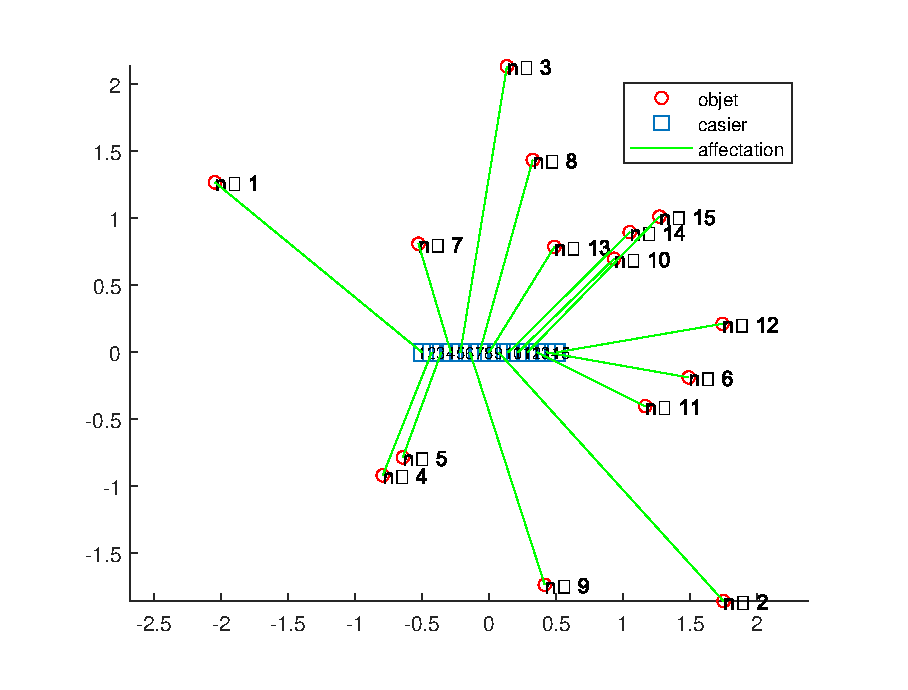
\includegraphics[scale=0.6]{figure/Q2.eps}
\caption{Solution of Question 2}
\label{fig:Q2}
\end{figure}



\subsection{A necessary condition for the solution}
For a solution, the affectation lines should not have intersections. Consider the following case in figure \ref{fig:Q2-nece}.

\begin{figure}[ht]
\centering
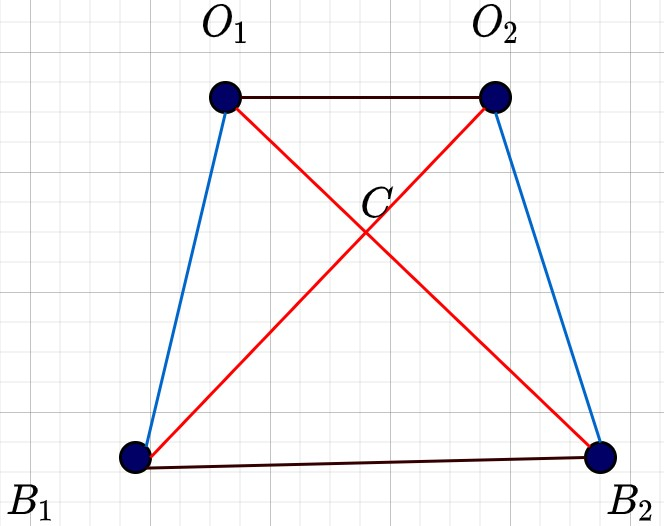
\includegraphics[scale=0.25]{figure/Q2-nece.jpg}
\caption{Illustrative example of the necessary condition}
\label{fig:Q2-nece}
\end{figure}

Suppose that the solution gives the red affectation lines, then $O_1B_1+O_2B_2\geqslant B_1O_2+B_2O_1$. However, according to the triangular inequality, we have $B_1O_2+B_2O_1=B_1C+CO_2+B_2C+CO_1 > O_1B_1+O_2B_2$. Therefore, there is a contradiction.



\section{Question 3}
\label{Q3}
As the object 1 can't be neither in box 1 nor in box $n$, we should have:
\begin{align}
    x_{1,1}=0\\
    x_{n,1}=0
\end{align}
So we simply need to modify the upper bound of $x_{1,1}$ and $x_{n,1}$ to 0.\par
The following code explain this process:
\begin{lstlisting}[style=MATLAB]
%% Q3
upper_bound(1)=0;
upper_bound(n)=0;
[x_tilde,fval]=linprog(c,[],[],L,ones(2*n,1),lower_bound,upper_bound);
Boxes=ConvPlot(x_tilde,n);
PlotSolution (Boxes, PositionsObjects, PositionsBoxes);
\end{lstlisting}
And we get the final result in figure \ref{fig:Q3}.
\begin{figure}[ht]
\centering
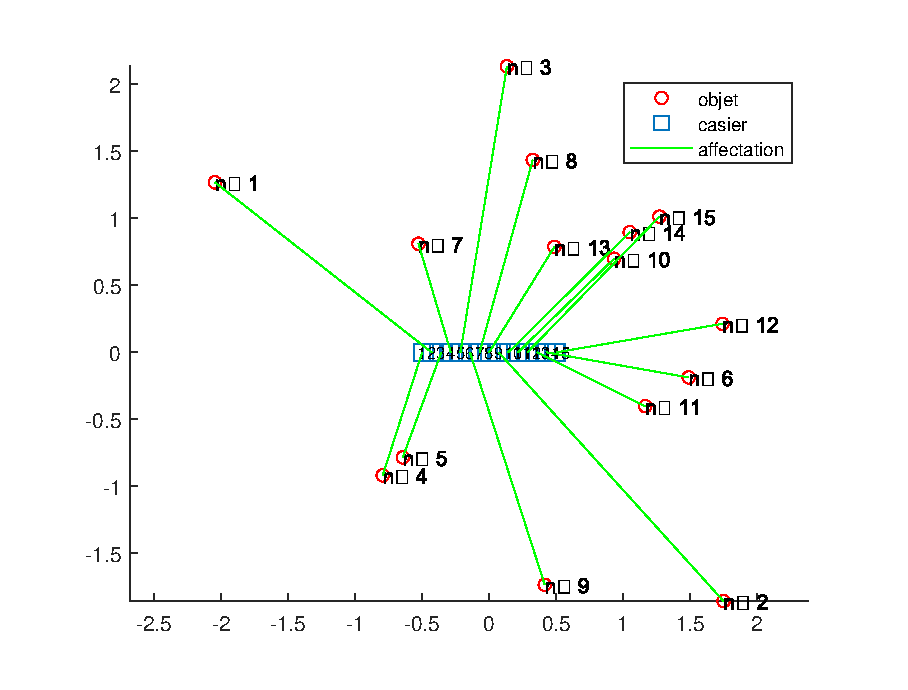
\includegraphics[scale=0.6]{figure/Q3.eps}
\caption{Solution of Question 3}
\label{fig:Q3}
\end{figure}

\section{Question 4}
\label{Q4}
The condition "object
2 must be in the box located just to the right of the box containing object 3" requires that:
if $x_{i,3}=1$,then $x_{i+1,2}=1$; if $x_{i,3}=0$,then $x_{i+1,2}=0$.\par
This can be explained as:
\begin{equation}
    \forall i\in \IntIntv{1}{n-1}, x_{i+1,2}-x_{i,3}=0
\end{equation}\par
We then try to explain this with the vector $\xtd$, we have:
\begin{equation}
    \left[\begin{matrix}
0^{(n-1)\times(n+1)}&\Ibb_{n-1}&-\Ibb_{n-1}&0^{(n-1)\times(n^2-3n+1)}
\end{matrix}\right]\xtd=0_{(n-1)\times 1}
\end{equation}
We the explain it to MATLAB code. 
\par {\color{red}Attention!This code just follows the code of section \ref{Q2-code} and all code of section \ref{Q3} shouldn't be executed!}
\begin{lstlisting}[style=MATLAB]
%Definition of L3
L3=[zeros(n-1,n+1),eye(n-1),-eye(n-1),zeros(n-1,n*n-3*n+1)];
L=[L;L3];
%Solve!
[x_tilde,fval]=linprog(c,[],[],L,[ones(2*n,1);zeros(n-1,1)],lower_bound,upper_bound);
Boxes=ConvPlot(x_tilde,n);
PlotSolution (Boxes, PositionsObjects, PositionsBoxes);
\end{lstlisting}
And this code gives the solution of figure \ref{fig:Q4}.
\begin{figure}[ht]
\centering
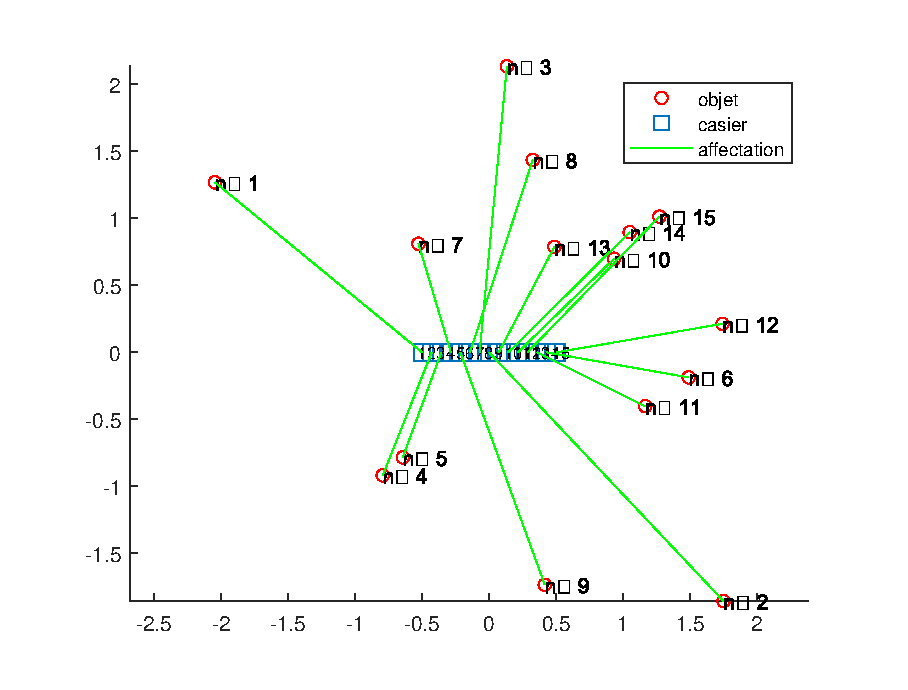
\includegraphics[scale=0.6]{figure/Q4.eps}
\caption{Solution of Question 4}
\label{fig:Q4}
\end{figure}

\section{Question 5}
\label{Q5}
The constraint $\forall i, x_{i,4}+\Sigma _{|k|\le 3}x_{i+k,5}\le 1$ means that there should be at least 3 boxes between the box containing object 4 and that containing object 5.\par
This gives the inequality constraints:
\begin{equation}
    A\tilde{x}\le \Onebb_{n}
\end{equation}
where
\begin{equation}
    A=\left[ \begin{matrix}
	0^{n\times 3n}&		I_n&		A_5&		0^{n\times 10n}\\
\end{matrix} \right] 
\end{equation}
\begin{equation}A_5=\left[\begin{matrix}
1&1&1&1&0&0&0&0&\cdots\\
1&1&1&1&1&0&0&0&\cdots\\
1&1&1&1&1&1&0&0&\cdots\\
1&1&1&1&1&1&1&0&\cdots\\
0&1&1&1&1&1&1&1&\cdots\\
\vdots& &\ddots&\ddots&\ddots&\ddots&\ddots&\ddots&\ddots\\
0&0&0&0&0&0&0&0&\cdots\\
0&0&0&0&0&0&0&0&\cdots\\
0&0&0&0&0&0&0&0&\cdots\\
0&0&0&0&0&0&0&0&\cdots\\
\end{matrix}
\begin{matrix}
0&0&0&0&0&0&0\\
0&0&0&0&0&0&0\\
0&0&0&0&0&0&0\\
0&0&0&0&0&0&0\\
0&0&0&0&0&0&0\\
\vdots&\vdots&\vdots&\vdots&\vdots&\vdots&\vdots\\
1&1&1&1&1&1&1\\
0&1&1&1&1&1&1\\
0&0&1&1&1&1&1\\
0&0&0&1&1&1&1\\
\end{matrix}\right]\end{equation}




By converting this into MATLAB code, we have:
\par {\color{red}Attention!This code just follows the code of section \ref{Q2-code} and all code of section \ref{Q3}, section \ref{Q4} shouldn't be executed!}
\begin{lstlisting}[style=MATLAB]
%% Q5
%Definition of A5
A5=[];
for i=1:n
    if i<=4
        A5=[A5;ones(1,i+3),zeros(1,n-(i+3))];
    else if i>=12
        A5=[A5;zeros(1,i-4),ones(1,n+4-i)];
        else
            A5=[A5;zeros(1,i-4),ones(1,7),zeros(1,n-i-3)];
        end
    end
end
A4=eye(15);
A=[zeros(n,3*n),A4,A5,zeros(n,10*n)];
b=ones(n,1);

%Solution
[x_tilde,fval]=intlinprog(c,1:(n*n),A,b,L,ones(2*n,1),lower_bound,upper_bound);
Boxes=ConvPlot(x_tilde,n);
PlotSolution (Boxes, PositionsObjects, PositionsBoxes);
\end{lstlisting}
And this code gives the solution of figure \ref{fig:Q5}.
\begin{figure}[ht]
\centering
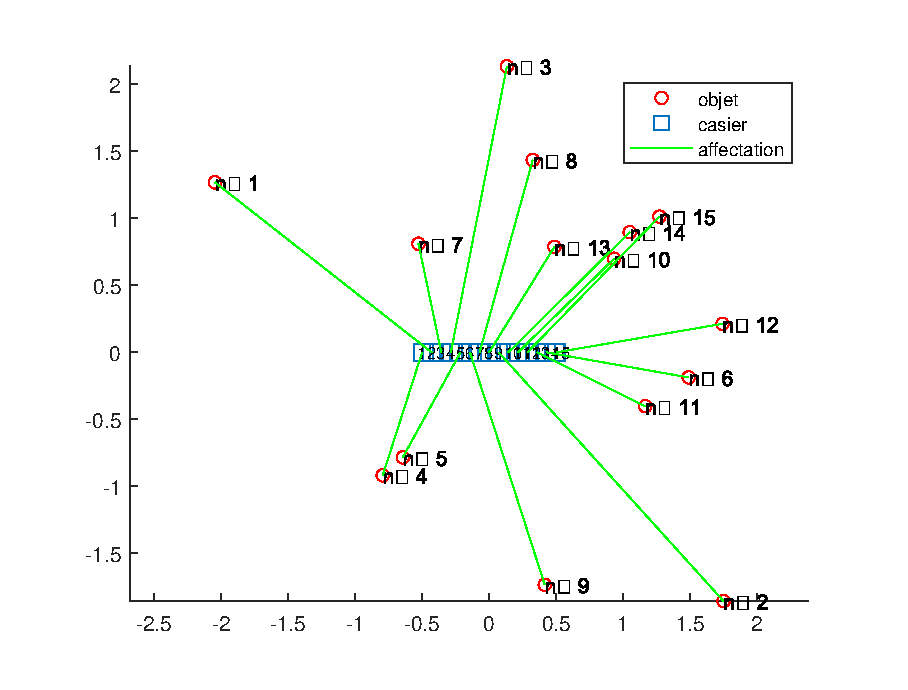
\includegraphics[scale=0.6]{figure/Q5.eps}
\caption{Solution of Question 5}
\label{fig:Q5}
\end{figure}

\section{Question 6}
\label{Q6}
Similarly, we can use the same formula as in section \ref{Q5}:
\begin{equation}
    \forall i, x_{i,6}-\Sigma _{|k|\le 3}x_{i+k,7} \le 0
\end{equation}.
\par
This gives the inequality constraints:
\begin{equation}
    A\tilde{x}\le 0_{n}
\end{equation}
where
\begin{equation}
    A=\left[ \begin{matrix}
	0^{n\times 5n}&		I_n&		-A_5&		0^{n\times 8n}\\
\end{matrix} \right] 
\end{equation}



By converting this into MATLAB code, we have:
\par {\color{red}Attention!This code just follows the code of section \ref{Q2-code} and all code of section \ref{Q3}, section \ref{Q4}, section \ref{Q5} shouldn't be executed!}
\begin{lstlisting}[style=MATLAB]
%Definition of A
A5=[];
for i=1:n
    if i<=4
        A5=[A5;ones(1,i+3),zeros(1,n-(i+3))];
    else if i>=12
        A5=[A5;zeros(1,i-4),ones(1,n+4-i)];
        else
            A5=[A5;zeros(1,i-4),ones(1,7),zeros(1,n-i-3)];
        end
    end
end
A6=eye(15);
A=[zeros(n,5*n),A6,-A5,zeros(n,8*n)];
b=zeros(n,1);

%Solution
[x_tilde,fval]=intlinprog(c,1:(n*n),A,b,L,ones(2*n,1),lower_bound,upper_bound);
Boxes=ConvPlot(x_tilde,n);
PlotSolution (Boxes, PositionsObjects, PositionsBoxes);
\end{lstlisting}
And this code gives the solution of figure \ref{fig:Q6}.
\begin{figure}[ht]
\centering
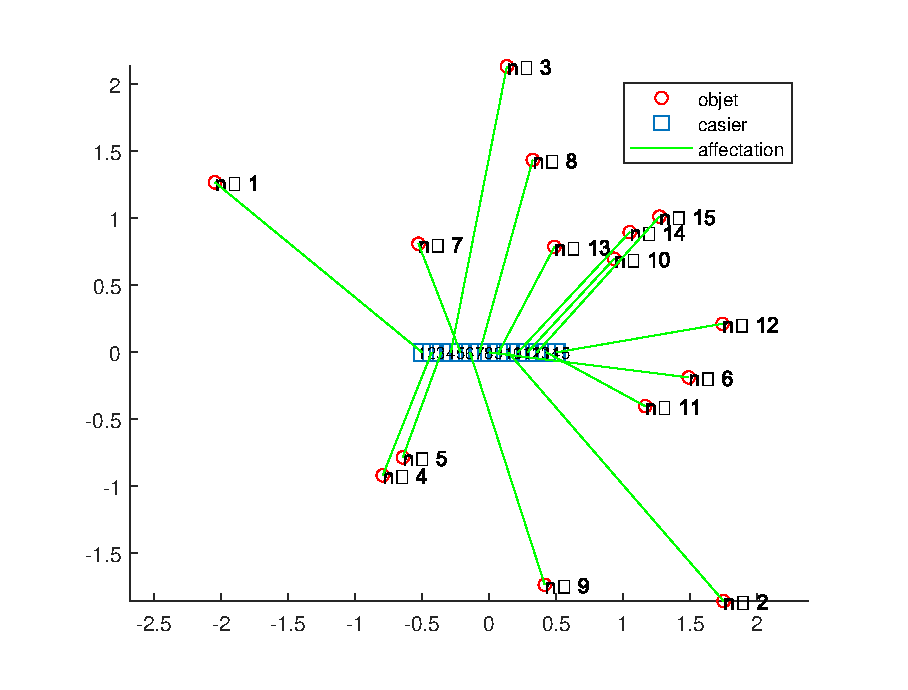
\includegraphics[scale=0.6]{figure/Q6.eps}
\caption{Solution of Question 6}
\label{fig:Q6}
\end{figure}


\section{Question 7}
\label{Q7}
\subsection{Strategy}
A simple strategy of verifying the uniqueness of solution is to delete the optimal solution from the feasible domain and try again to solve this question. We see if we can get again the same optimal value.\par
As we know that there will only be $n$ position in $\xtd$ that the value is 1, other values are all 0. To delete this optimal solution, a simple strategy for this question is to make a scalar product with this solution. If the new optimal solution is the same as the older one, it's not unique. Othervise it's unique.\par
More precisely, we have the original optimization question $\Qcal$:
\begin{equation*}
        \min_{\xtd \in \{0,1\}^{n^2\times 1}} <\cbs|\xtd> \quad \st  \quad A \xtd \le \bbs, L\xtd= \dbs
\end{equation*}
And it gives an optimal solution $\xtd_1$ with $f_1=<\cbs|\xtd_1>$.
Then we solve again this question, with additional constrains:
\begin{equation*}
        \min_{\xtd \in \{0,1\}^{n^2\times 1}} <\cbs|\xtd> \quad \st  \quad \left[\begin{matrix}A\\\xtd_1^{T}\end{matrix}\right] \xtd \le \left[\begin{matrix}\bbs\\n-1\end{matrix}\right], L\xtd= \dbs
\end{equation*}
And we see if the solution gives $f_2=f_1$
\subsection{Test result on $\Pcal_2$}
We process this strategy on $\Pcal_2$. We remind that the section \ref{Q4} gives a solution as in figure \ref{fig:Q4} and the optimal value is $20.5341$.Imagine the original optimal solution is \verb|x_tilde1|, we execute:
\par {\color{red}Attention!This code just follows the code of section \ref{Q4} and all other codes shouldn't be executed!}
\begin{lstlisting}[style=MATLAB]
%New solution
A=x_tilde1';
b=n-1;
[x_tilde2,fval2]=intlinprog(c,1:n^2,A,b,L,[ones(2*n,1);zeros(n-1,1)],lower_bound,upper_bound);
%examine
if abs(fval1-fval2)<1e-5
    disp('not unique');
    Boxes=ConvPlot(x_tilde1,n);
    PlotSolution (Boxes, PositionsObjects, PositionsBoxes);

    Boxes=ConvPlot(x_tilde2,n);
    PlotSolution (Boxes, PositionsObjects, PositionsBoxes);
else
    disp('unique');
end
\end{lstlisting}
And it gives the answer 'unique', with the new optimal solution $20.5343>20.5341$.

\subsection{Test result on $\Pcal_3$}
We process this strategy on $\Pcal_3$. We remind that the section \ref{Q5} gives a solution as in figure \ref{fig:Q5} and the optimal value is $20.5816$. Imagine the original optimal solution is \verb|x_tilde1|, we execute:
\par {\color{red}Attention!This code just follows the code of section \ref{Q5} and all other codes shouldn't be executed!}
\begin{lstlisting}[style=MATLAB]
%New solution
A=[A;x_tilde1'];
b=[b;n-1];

[x_tilde2,fval2]=intlinprog(c,1:(n*n),A,b,L,ones(2*n,1),lower_bound,upper_bound);
%examine
if abs(fval1-fval2)<1e-5
    disp('not unique');
    Boxes=ConvPlot(x_tilde1,n);
    PlotSolution (Boxes, PositionsObjects, PositionsBoxes);

    Boxes=ConvPlot(x_tilde2,n);
    PlotSolution (Boxes, PositionsObjects, PositionsBoxes);
else
    disp('unique');
end

\end{lstlisting}
And it gives the new optimal solution $20.5816$. So this solution isn't unique. We have another solution proposed as in the figure \ref{fig:Q7}.
\begin{figure}[ht]
\centering
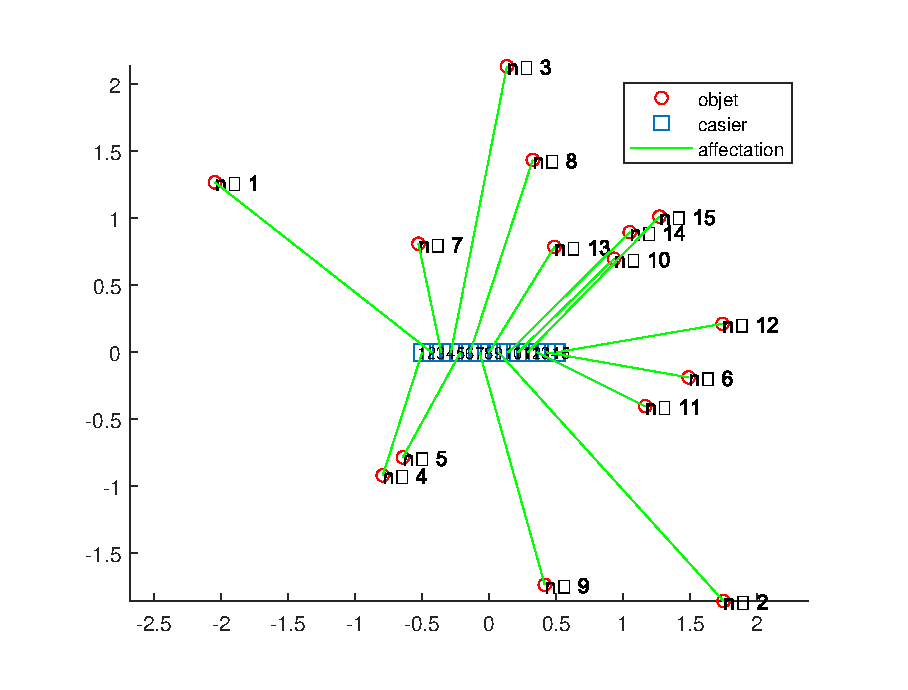
\includegraphics[scale=0.6]{figure/Q7.eps}
\caption{Another Optimal Solution of Question 5}
\label{fig:Q7}
\end{figure}

\section{Comment on linprog and intlinprog}
It can be easily verified that the matrices $L$ in the questions 2,3,4 are TUM. According to the course, the solutions delivered by the simplex to the corresponding LP problems are in $\{0,1\}^{n^2}$. Therefore, the solutions are also the solutions of the corresponding ILP problems. That's why we could use the Matlab function \verb|linprog| instead of \verb|intlinprog|.
\end{document}
